Cinco filósofos se encuentran sentados en una mesa redonda con una fuente de arroz en el centro, entre cada 
par de filósofos se encuentra un palillo, sumando 5 en total. \\
Para que un filósofo pueda comer, debe poder obtener en forma exclusiva dos palillos, el que se encuentra 
a su izquierda y el que se encuentra a su derecha. El objetivo del algorítmo es lograr que todos los 
filósofos puedan comer sin que ninguno muera por inanición. La inanici\'on se produce cuando un filósofo logra obtener 
un solo cubierto, no pudiendo obtener el segundo, el cual está en manos de otro filósofo que espera obtener 
el cubierto del primero.

\begin{figure}[!h]
	\centering
	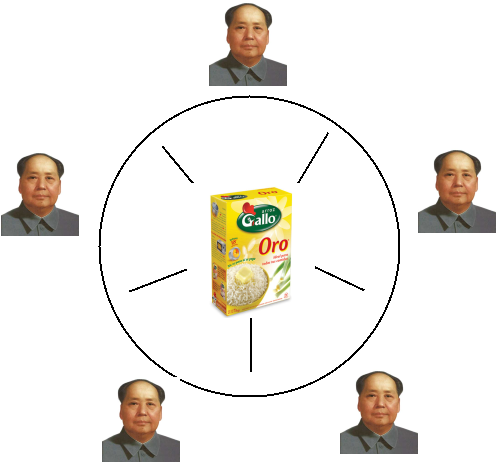
\includegraphics[scale=0.4]{secciones/imagenes/chinos.png}
	\caption{Problema de los fil\'osofos chinos}
	\label{fig:filosofos}
\end{figure}

\subsection{Arquitectura}
El problema será resuelto utilizando un servicio de semáforos implementado en el \emph{MM}.  Se utilizará 
un arreglo global para guardar el estado de cada filósofo, pudiendo ser accedido por todos los procesos involucrados 
(uno por cada filósofo).  El servicio de memoria compartida ha sido implementado también en el \emph{MM},
tal cual fue descrito anteriormente.
\subsection{Algorítmo}
MIRAR - PONER ALGUNA GILADA

\subsubsection{Global - Inicialización}
Inicialización de un semaforo bloqueante por filosofo. Los semaforos son inicializados en -1,
lo cual provoca que la proxima llamada a $P(X)$ bloqueé al proceso invocante (autobloqueo).
Por otro lado, se inicializan los estados de todos los filósofos a {\bf PENSANDO}.
Finalmente, se crear\'a el mutex que permitirá el acceso exclusivo al array de estados por parte de cada proceso.

\begin{scriptsize} 
\begin{verbatimtab} 
	Para i = 1 Hasta MAX_FILOSOFOS
		crear (S(i))
		P(S(i))
		Estado(i) = PENSANDO
	Fin Para
	crear(mutex)
	IniciarProcesos()	
\end{verbatimtab}
\end{scriptsize}

\subsubsection{Filosofo i - Ciclo Principal}
El siguiente es el ciclo principal que ejecuta el proceso del filósofo $i$. El ciclo comienza en el estado {\bf PENSANDO}. 
En algún momento, dicho estado termina y es necesario evaluar si se puede pasar directamente a 
{\bf COMIENDO} o si es necesario esperar los cubiertos.  En este segundo caso, el proceso queda bloqueado 
hasta tanto algún proceso vecino le avise de la disponibilidad de los mismos. Finalmente, para ambos 
casos el proceso pasará al estado {\bf COMIENDO} y, al terminar este, avisará a los procesos vecinos 
de la disponibilidad de los cubiertos.

\begin{scriptsize} 
\begin{verbatimtab} 
	LoopForEver
		Pensar()			
		P(mutex)			        // Obtiene acceso exclusivo a los estados
		Si !testear(i, false)		// Verifica si puede comer. 
			Estado(i) = ESPERANDO	// No puede, se pone en espera
			V(mutex)
			P(S(i))			        // Autobloqueo
		Sino
			V(mutex)
		Fin Si		
		// Este punto puede ser alcanzado de dos maneras: 
		// 1. La llamada testear(i, false) dio true, lo cual significa que 
		// el filósofo podía comer en ese momento
		// 2. El proceso había sido autobloqueado, pero otro lo despertó.
		Comer()
		largar(i)                   // Avisa que los cubiertos están ahora libres
	End Loop
\end{verbatimtab}
\end{scriptsize}

\subsubsection{Filosofo i - Función Testear}
La función testear tiene el siguiente prototipo:

\begin{scriptsize} 
\begin{verbatimtab} 
	bool testear(int idFilosofo, bool isWakeUp) 
\end{verbatimtab}
\end{scriptsize}

El argumento $isWakeUp$ indica la modalidad de llamada a la función. Cuando se pasa en $false$, 
el testeo está siendo realizado por el mismo proceso que la invoca. Cuando el argumento es $true$, se 
está despertando a otro proceso bloqueado, en caso de estar presente la posibilidad de comer 
para el mismo (podría pasar que el otro proceso vecino tenga el otro cubierto). 
La función devolverá $true$ si es posible comer o $false$ en caso contrario.

\begin{scriptsize} 
\begin{verbatimtab} 
	func bool testear(int idFilosofo, bool isWakeUp)
		// Esta guarda verifica las condiciones bajo las que se tienen que ejecutar
		// los tests. 
		Si (Estado(i) == ESPERANDO And isWakeUp) Or (Estado(i) == PENSANDO And !isWakeUp) then
			// Verifica que los vecinos no estén comiendo
			Si Estado(LEFT(i)) != COMIENDO And Estado(RIGHT(i)) != COMIENDO then
				Si isWakeUp Then	// Solo desbloquear si ya estaba bloqueado			
					V(i)
				return(true)		
			Sino
				return(false)		// Si no puede comer no se debe desbloquear
		Fin Si	
	end func
\end{verbatimtab}
\end{scriptsize}

\subsubsection{Filosofo i - Función Largar}
La función $largar(i)$ tiene como fin permitir a un proceso notificar a sus vecinos que los cubiertos 
que acaba de utilizar están nuevamente disponibles. Para esto, se ejecuta la función testear 
en modo $wakeUp$ sobre el vecino izquierdo y el derecho.  La señal de desbloqueo será enviada a 
un vecino solamente cuando el testeo sea exitoso.

\begin{scriptsize} 
\begin{verbatimtab} 
	func void largar(int idFilosofo)
		P(mutex)
		Estado(i) = PENSANDO
		testear(LEFT(i), true)
		testear(RIGHT(i), true)
		V(mutex)
	end func
\end{verbatimtab}
\end{scriptsize}

\subsection{Localización del código y ejemplos}
El código MINIX para este ejercicio se encuentra en el directorio $/usr/tp/14$. Existe un solo archivo 
fuente,  $/usr/tp/14/filo.c$, el cual puede ser parametrizado con la variable \emph{MAX\_PROCS} para
variar la cantidad de procesos concurrentes. El shell script $compex$ producir\'a los ejecutables $fex1$, 
$fex2$ y $fex3$, los cuales corresponden a los siguientes ejemplos:

\subsubsection{Ejemplo 1 - 2 Fil\'osofos ($fex1$)}

Este ejemplo tiene como finalidad mostrar que bajo el algoritmo implementado dos fil\'osofos vecinos se exluyen 
mutuamente. Si se da la oportunidad (segun variables temporales) tambie'n se \textit{desbloquear\'an} mutuamente.
La traza se ve de la siguiente manera, pero debe tenerse en cuenta que la misma ha sido depurada
dado que el orden en que aparecen los mensajes en la consola no es necesariamente el mismo que
en el que ocurren los eventos (lo que queremos destacar aquí es la exclusio'on mutua la cual puede observarse
en los registros del tipo : 1[ESTADO\_1].....N[ESTADO\_N]. La misma observaºci\'on aplica para el resto de los ejemplos.

\begin{scriptsize} 
\begin{verbatimtab} 
[1][PENS]  [2][COMI]  
[F2] Pensado...
[1][COMI]  [2][ESPE]  
[F2] Comiendo...
[1][PENS]  [2][PENS]  
[F2] Pensado...
[1][COMI]  [2][ESPE]  
[F2] Comiendo...
[1][PENS]  [2][PENS]  
[F2] Pensado...
[1][COMI]  [2][ESPE]  
[F2] Comiendo...
[1][PENS]  [2][PENS]  
[F2] Pensado...
[1][COMI]  [2][ESPE]  
[F2] Comiendo...
\end{verbatimtab}
\end{scriptsize}

\subsubsection{Ejemplo 2 - 3 Fil\'osofos ($fex2$)}
Este ejemplo es basicamente una consecuencia del primero. En el mismo puede apreciarse que, al 
haber 3 filosofos en total, cada uno con 2 vecinos, solo es posible que coma una a la vez.

\begin{scriptsize} 
\begin{verbatimtab} 
[1][PENS]  [2][ESPE]  [3][PENS]  
[1][PENS]  [2][COMI]  [3][PENS]  
[1][PENS]  [2][PENS]  [3][COMI]  
[1][PENS]  [2][PENS]  [3][PENS]  
[1][PENS]  [2][PENS]  [3][PENS]  
[1][PENS]  [2][ESPE]  [3][COMI]  
[1][ESPE]  [2][PENS]  [3][ESPE]  
[1][COMI]  [2][PENS]  [3][ESPE]  
[1][COMI]  [2][ESPE]  [3][ESPE]  
[1][ESPE]  [2][PENS]  [3][ESPE]  
[1][COMI]  [2][PENS]  [3][ESPE]  
\end{verbatimtab}
\end{scriptsize}
\subsubsection{Ejemplo 3 - 4 Fil\'osofos ($fex3$)}
En este ejemplo se muestra que los vecinos no contiguos no son mutuamente excluyentes. Por lo tanto,
podrań comer simultaneamente los del grupo ''par'' o ''impar'', pero no ambos grupos a la vez.

\begin{scriptsize} 
\begin{verbatimtab} 
[1][PENS]  [2][PENS]  [3][PENS]  [4][PENS]  
[1][PENS]  [2][COMI]  [3][ESPE]  [4][COMI]  <----
[1][ESPE]  [2][PENS]  [3][ESPE]  [4][PENS]  
[1][COMI]  [2][PENS]  [3][ESPE]  [4][PENS]  
[1][COMI]  [2][PENS]  [3][COMI]  [4][PENS]  
[1][COMI]  [2][ESPE]  [3][PENS]  [4][ESPE]  
[1][PENS]  [2][PENS]  [3][ESPE]  [4][PENS]  
[1][PENS]  [2][PENS]  [3][COMI]  [4][PENS]  
[1][COMI]  [2][ESPE]  [3][PENS]  [4][ESPE]  
[1][PENS]  [2][PENS]  [3][ESPE]  [4][PENS]  
[1][PENS]  [2][PENS]  [3][PENS]  [4][PENS]  
[1][PENS]  [2][PENS]  [3][PENS]  [4][PENS]  
[1][PENS]  [2][PENS]  [3][PENS]  [4][PENS]  
[1][PENS]  [2][PENS]  [3][PENS]  [4][COMI]  
[1][ESPE]  [2][COMI]  [3][ESPE]  [4][PENS]  
[1][COMI]  [2][PENS]  [3][COMI]  [4][ESPE]  
[1][PENS]  [2][COMI]  [3][PENS]  [4][PENS] <---- 
[1][COMI]  [2][PENS]  [3][COMI]  [4][ESPE]  
[1][PENS]  [2][COMI]  [3][PENS]  [4][PENS]   
\end{verbatimtab}
\end{scriptsize}

